\documentclass[14pt]{extarticle}

\usepackage[table]{xcolor} % colored lines for tables
\usepackage[normalem]{ulem} % strike through text
\usepackage{amsmath,mathtools,amsfonts,amsthm,amssymb,hyperref}
\usepackage{parskip,geometry,latexsym,bookmark,mathtools,float,cancel}
\usepackage{minted,tcolorbox,bm}

\usepackage[mathscr]{euscript}
\let\euscr\mathscr
\let\mathscr\relax
\usepackage[scr]{rsfso}
\newcommand{\ps}{\mathscr{P}} % for the Power set P

\newtheorem{defn}{Definition}
\newtheorem{thm}{Theorem}
\newtheorem{claim}{Claim}
\newtheorem{lemma}{Lemma}

\newcommand{\dps}{\displaystyle}
\newcommand{\es}{\varnothing}
\newcommand{\fbl}{\underline{\hspace{1cm}}\,\,}
\newcommand{\R}{\mathbb{R}}
\newcommand{\Q}{\mathbb{Q}}
\newcommand{\Z}{\mathbb{Z}}
\newcommand{\from}{\leftarrow}
\newcommand{\true}{{\bf t}}
\newcommand{\false}{{\bf c}}
\newcommand{\bic}{\leftrightarrow}
\newcommand{\da}{\downarrow}
\newcommand{\fa}{\forall}
\newcommand{\te}{\exists}
\newcommand{\cy}{\color{cyan}}

\newcommand{\colsq}[1]{{\color{#1} $\blacksquare$}}

\newcommand{\base}[1]{{\cy #1}} % for log bases
\newcommand{\floor}[1]{{\left\lfloor#1\right\rfloor}}
\newcommand{\ceil}[1]{{\left\lceil#1\right\rceil}}
\newcommand\Ccancel[2][black]{\renewcommand\CancelColor{\color{#1}}\cancel{#2}}
\newcommand\Cbcancel[2][black]{\renewcommand\CancelColor{\color{#1}}\bcancel{#2}}

\renewcommand{\arraystretch}{1.2}

\hypersetup{colorlinks,allcolors=blue,linktoc=all}
\geometry{a4paper}
\geometry{margin=0.42in}

\title{Solutions to Chapter 8, Susanna Epp Discrete Math 5th Edition}

\author{https://github.com/spamegg1}

\begin{document}
\maketitle
\tableofcontents


\section{Exercise Set 8.1}

\subsection{Exercise 1}
As in Example 8.1.2, the {\bf congruence modulo 2} relation $E$ is defined from $\Z$ to $\Z$ as follows: For every 
ordered pair \((m, n) \in \Z \times \Z\), $m$ $E$ $n$ \(\iff m - n\) is even.

\subsubsection{(a)}
Is $0$ $E$ $0$? Is $5$ $E$ $2$? Is $(6, 6) \in E$? Is $(21, 7) \in E$?

\begin{proof}
$0$ $E$ $0$ because \(0 - 0 = 0 = 2 \cdot 0\), so \(2 \mid (0 - 0)\). $5$ $\Ccancel{E}$ $2$ because \(5 - 2 = 3\) and 
\(3 \neq 2k\) for any integer $k$, so \(2 \nmid (5 - 2)\). \((6, 6) \in E\) because \(6 - 6 = 0 = 2 \cdot 0\), so \(2 
\mid (6 - 6). (-1, 7) \in E\) because \(-1 - 7 = -8 = 2 \cdot (-4)\), so \(2 \mid (-1 - 7)\).
\end{proof}

\subsubsection{(b)}
Prove that for any even integer $n$, $n$ $E$ $0$.

\begin{proof}
Assume $n$ is even. By definition of even, $n=2k$ for some integer $k$. Then \(n - 0 = 2k - 0 = 2k\) is also even.
Therefore by definition of $E$, $n$ $E$ 0.
\end{proof}

\subsection{Exercise 2}
Prove that for all integers $m$ and $n$, $m - n$ is even if, and only if, both $m$ and $n$ are even or both $m$ and 
$n$ are odd.

\begin{proof}
\(\bm{\implies}\): Assume $m-n$ is even. {\it [We want to prove that both $m$ and $n$ are even or both $m$ and $n$ 
are odd.]} By definition of even, \(m - n = 2k\) for some integer $k$. There are 4 cases:

{\bf Case 1: both $m$ and $n$ are even:} Nothing to prove.

{\bf Case 2: both $m$ and $n$ are odd:} Nothing to prove.

{\bf Case 3: $m$ is even, $n$ is odd:} By definitions of even and odd, \(m=2k, n=2l+1\) for some integers $k,l$. 
So \(m-n = 2k-2l-1 = 2(k-l-1) + 1\) where \(k-l-1\) is an integer. So by definition of odd, \(m-n\) is odd, a 
contradiction. So this case is impossible.

{\bf Case 4: $m$ is odd, $n$ is even:} By definitions of even and odd, \(m=2k+1, n=2l\) for some integers $k,l$. 
So \(m-n = 2k+1-2l = 2(k-l) + 1\) where \(k-l\) is an integer. So by definition of odd, \(m-n\) is odd, a 
contradiction. So this case is impossible.

\(\bm{\impliedby}\): Assume both $m$ and $n$ are even or both $m$ and $n$ are odd. {\it [We want to prove that $m-n$ 
is even.]} There are 2 cases:

{\bf Case 1: both $m$ and $n$ are even:} By definition of even, \(m = 2k, n = 2l\) for some integers $k,l$. Then 
\(m-n = 2k-2l = 2(k-l)\) where $k-l$ is an integer. So by definition, $m-n$ is even.

{\bf Case 2: both $m$ and $n$ are odd:} By definition of even, \(m = 2k+1, n = 2l+1\) for some integers $k,l$. Then 
\(m-n = 2k+1-2l-1 = 2(k-l)\) where $k-l$ is an integer. So by definition, $m-n$ is even.
\end{proof}

\subsection{Exercise 3}
The congruence modulo 3 relation, $T$, is defined from $\Z$ to $\Z$ as follows: For all integers $m$ and $n$, $m$ $T$ 
$n$ \(\iff 3 \mid (m - n)\).

\subsubsection{(a)}
Is $10$ $T$ $1$? Is $1$ $T$ $10$? Is \((2, 2) \in T\)? Is \((8, 1) \in T\)?

\begin{proof}
10 $T$ 1 because \(10 - 1 = 9 = 3 \cdot 3\), and so \(3 \mid (10 - 1)\).

1 $T$ 10 because \(1 - 10 = -9 = 3 \cdot (-3)\), and so \(3 \mid (1 - 10)\).

2 $T$ 2 because \(2 - 2 = 0 = 3 \cdot 0\), and so \(3 \mid (2 - 2)\).

8 $\Ccancel{T}$ 1 because \(8 - 1 = 7 \neq 3k\), for any integer $k$. So \(3 \nmid (8 - 1)\).
\end{proof}

\subsubsection{(b)}
List five integers $n$ such that $n$ $T$ $0$.

\begin{proof}
One possible answer: 3, 6, 9, $-3$, $-6$
\end{proof}

\subsubsection{(c)}
List five integers $n$ such that $n$ $T$ 1.

\begin{proof}
One possible answer: 4, 7, 10, $-2$, $-5$
\end{proof}

\subsubsection{(d)}
List five integers $n$ such that $n$ $T$ $2$.

\begin{proof}
One possible answer: 5, 8, 11, $-1$, $-4$
\end{proof}

\subsubsection{(e)}
Make and prove a conjecture about which integers are related by $T$ to $0$, which integers are related by $T$ to 
1, and which integers are related by $T$ to 2.

All integers of the form \(3k + 1\), for some integer $k$, are related by $T$ to $1$.

\begin{proof}
All integers of the form \(3k\), for some integer $k$, are related by $T$ to 0.

All integers of the form \(3k+1\), for some integer $k$, are related by $T$ to 1.

All integers of the form \(3k+2\), for some integer $k$, are related by $T$ to 2.
\end{proof}

\subsection{Exercise 4}
Define a relation $P$ on $\Z$ as follows: For every ordered pair \((m, n) \in \Z \times \Z\), $m$ $P$ $n$ \(\iff\) $m$ 
and $n$ have a common prime factor.

\subsubsection{(a)}
Is 15 $P$ 25?

\begin{proof}
Yes, because 15 and 25 are both divisible by 5, which is prime.
\end{proof}

\subsubsection{(b)}
Is 22 $P$ 27?

\begin{proof}
No, because 22 and 27 have no common prime factor.
\end{proof}

\subsubsection{(c)}
Is 0 $P$ 5?

\begin{proof}
Yes, because 0 and 5 are both divisible by 5, which is prime.
\end{proof}

\subsubsection{(d)}
Is 8 $P$ 8?

\begin{proof}
Yes, because 8 and 8 are both divisible by 2, which is prime.
\end{proof}

\subsection{Exercise 5}
Let \(X = \{a, b, c\}\). Recall that \(\ps(X)\) is the power set of $X$. Define a relation {\bf S} on \(\ps(X)\) 
as follows: For all sets $A$ and $B$ in \(\ps(X)\), $A$ {\bf S} $B$ $\iff$ $A$ has the same number of elements as $B$.

\subsubsection{(a)}
Is \(\{a, b\}\) {\bf S} \(\{b, c\}\)?

\begin{proof}
Yes, because both \(\{a, b\}\) and \(\{b, c\}\) have two elements.
\end{proof}

\subsubsection{(b)}
Is \(\{a\}\) {\bf S} \(\{a,b\}\)?

\begin{proof}
No, one has 1 element, the other has 2 elements.
\end{proof}

\subsubsection{(c)}
Is \(\{c\}\) {\bf S} \(\{b\}\)?

\begin{proof}
Yes, because both \(\{c\}\) and \(\{b\}\) have one element.
\end{proof}

\subsection{Exercise 6}
Let \(X = \{a, b, c\}\). Define a relation {\bf J} on \(\ps(X)\) as follows: For all sets $A$ and $B$ in $\ps(X)$,
$A$ {\bf J} $B$ $\iff$ \(A \cap B \neq \es\).

\subsubsection{(a)}
Is $\{a\}$ {\bf J} $\{c\}$?

\begin{proof}
No, because \(\{a\} \cap \{c\} = \es\).
\end{proof}

\subsubsection{(b)}
Is $\{a, b\}$ {\bf J} $\{b, c\}$?

\begin{proof}
Yes, because \(\{a,b\} \cap \{b,c\} = \{b\} \neq \es\).
\end{proof}

\subsubsection{(c)}
Is $\{a, b\}$ {\bf J} $\{a, b, c\}$?

\begin{proof}
Yes, because \(\{a,b\} \cap \{a,b,c\} = \{a,b\} \neq \es\).
\end{proof}

\subsection{Exercise 7}
Define a relation $R$ on $\Z$ as follows: For all integers $m$ and $n$, $m$ $R$ $n$ $\iff$ \(5 \mid (m^2 - n^2)\).

\subsubsection{(a)}
Is 1 $R$ $(-9)$?

\begin{proof}
Yes. 1 $R$ \((-9) \iff 5 \mid (1^2 - (-9)^2)\). But \(1^2 - (-9)^2 = 1 - 81 = -80\), and \(5 \mid (-80)\) because 
\(-80 = 5 \cdot (-16)\).
\end{proof}

\subsubsection{(b)}
Is 2 $R$ 13?

\begin{proof}
Yes, \(2^2 - (13)^2 = 4 - 169 = -165 = 5 \cdot (-33)\). So \(5 \mid 2^2 - (13)^2\).
\end{proof}

\subsubsection{(c)}
Is 2 $R$ $(-8)$?

\begin{proof}
Yes, \(2^2 - (-8)^2 = 4 - 64 = -60 = 5 \cdot (-12)\). So \(5 \mid 2^2 - (-8)^2\).
\end{proof}

\subsubsection{(d)}
Is $(-8)$ $R$ 2?

\begin{proof}
Yes, \((-8)^2 - 2^2 = 64 - 4 = 60 = 5 \cdot 12\). So \(5 \mid (-8)^2 - 2^2\).
\end{proof}

\subsection{Exercise 8}
Let $A$ be the set of all strings of $a$’s and $b$’s of length 4. Define a relation $R$ on $A$ as follows: For 
every \(s, t \in A\), $s$ $R$ $t$ $\iff$ $s$ has the same first two characters as $t$.

\subsubsection{(a)}
Is $abaa$ $R$ $abba$?

\begin{proof}
Yes, because both $abaa$ and $abba$ have the same first two characters $ab$.
\end{proof}

\subsubsection{(b)}
Is $aabb$ $R$ $bbaa$?

\begin{proof}
No, because the first two characters of $aabb$ are different from the first two characters of $bbaa$.
\end{proof}

\subsubsection{(c)}
Is $aaaa$ $R$ $aaab$?

\begin{proof}
Yes, because both $aaaa$ and $aaab$ have the same first two characters $aa$.
\end{proof}

\subsubsection{(d)}
Is $baaa$ $R$ $abaa$?

\begin{proof}
No, because the first two characters of $baaa$ are different from the first two characters of $abaa$.
\end{proof}

\subsection{Exercise 9}
Let $A$ be the set of all strings of 0’s, 1’s, and 2’s of length 4. Define a relation $R$ on $A$ as follows: For 
every \(s, t \in A\), $s$ $R$ $t$ $\iff$ the sum of the characters in $s$ equals the sum of the characters in $t$.

\subsubsection{(a)}
Is 0121 $R$ 2200?

\begin{proof}
Yes, because the sum of the characters in 0121 is 4 and the sum of the characters in 2200 is also 4.
\end{proof}

\subsubsection{(b)}
Is 1011 $R$ 2101?

\begin{proof}
No, because the sum of the characters in 1011 is 3, whereas the sum of the characters in 2101 is 4.
\end{proof}

\subsubsection{(c)}
Is 2212 $R$ 2121?

\begin{proof}
No, because the sum of the characters in 2212 is 7, whereas the sum of the characters in 2121 is 6.
\end{proof}

\subsubsection{(d)}
Is 1220 $R$ 2111?

\begin{proof}
Yes, because the sum of the characters in 1220 is 5 and the sum of the characters in 2111 is also 5.
\end{proof}

\subsection{Exercise 10}
Let \(A = \{3, 4, 5\}\) and \(B = \{4, 5, 6\}\) and let $R$ be the “less than” relation. That is, for every ordered 
pair \((x, y) \in A \times B, x \, R \, y \iff x < y\). State explicitly which ordered pairs are in $R$ and $R^{-1}$.

\begin{proof}
\(R = \{(3, 4), (3, 5), (3, 6), (4, 5), (4, 6), (5, 6)\}\)

\(R^{-1} = \{(4, 3), (5, 3), (6, 3), (5, 4), (6, 4), (6, 5)\}\)
\end{proof}

\subsection{Exercise 11}
Let \(A = \{3, 4, 5\}\) and \(B = \{4, 5, 6\}\) and let $S$ be the “divides” relation. That is, for every ordered pair 
\((x, y) \in A \times B, x \, S \, y \iff x \mid y\). State explicitly which ordered pairs are in $S$ and $S^{-1}$.

\begin{proof}
\(S = \{(3, 6), (4, 4), (5, 5)\}, S^{-1} = \{(6, 3), (4, 4), (5, 5)\}\)
\end{proof}

\subsection{Exercise 12}

\subsubsection{(a)}
Suppose a function \(F: X \to Y\) is one-to-one but not onto. Is \(F^{-1}\) (the inverse relation for $F$) a 
function? Explain your answer.

\begin{proof}
No. If \(F: X \to Y\) is not onto, then $F$ fails to be defined on all of $Y$. In other words, there is an element 
$y$ in $Y$ such that \((y, x) \notin F^{-1}\) for any \(x \in X\). Consequently, \(F^{-1}\) does not satisfy property 
(1) of the definition of function.
\end{proof}

\subsubsection{(b)}
Suppose a function \(F: X \to Y\) is onto but not one-to-one. Is \(F^{-1}\) (the inverse relation for $F$) a 
function? Explain your answer.

\begin{proof}
No. If \(F: X \to Y\) is not one-to-one, then $F$ for some $y$ in $Y$, there will be multiple potential values for 
\(F^{-1}(y)\). In other words, there is an element $y$ in $Y$ and elements \(x_1, x_2 \in X\) such that \((y, x_1) 
\in F^{-1}\) and \((y, x_2) \in F^{-1}\). Consequently, \(F^{-1}\) does not satisfy property (2) of the definition 
of function.
\end{proof}

{\bf \cy Draw the directed graphs of the relations defined in $13-18$.}

\subsection{Exercise 13}
Define a relation $R$ on \(A = \{0, 1, 2, 3\}\) by \(R = \{(0, 0), (1, 2), (2, 2)\}\).

\begin{proof}
\begin{figure}[ht!]
\centering
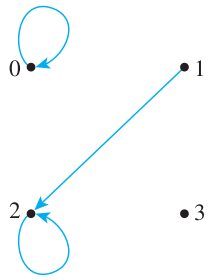
\includegraphics[scale=0.4]{../images/8.1.13.png}
\end{figure}
\end{proof}

\subsection{Exercise 14}
Define a relation $S$ on \(B = \{a, b, c, d\}\) by \(S = \{(a, b), (a, c), (b, c), (d, d)\}\).

\begin{proof}
\begin{figure}[ht!]
\centering
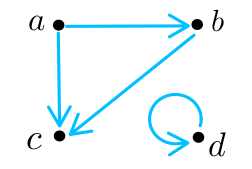
\includegraphics[scale=0.4]{../images/8.1.14.png}
\end{figure}
\end{proof}

\subsection{Exercise 15}
Let \(A = \{2, 3, 4, 5, 6, 7, 8\}\) and define a relation $R$ on $A$ as follows: For every \(x, y \in A, x \, R\, y 
\iff x \mid y\).

\begin{proof}
\begin{figure}[ht!]
\centering
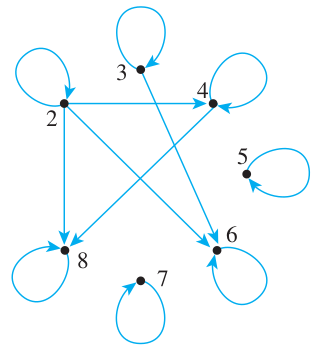
\includegraphics[scale=0.4]{../images/8.1.15.png}
\end{figure}
\end{proof}

\subsection{Exercise 16}
Let \(A = \{5, 6, 7, 8, 9, 10\}\) and define a relation $S$ on $A$ as follows: For every \(x, y \in A, x \, S \, y \iff 
2 \mid (x - y)\).

\begin{proof}
\begin{figure}[ht!]
\centering
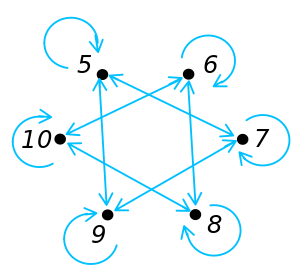
\includegraphics[scale=0.4]{../images/8.1.16.png}
\end{figure}
\end{proof}

\subsection{Exercise 17}
Let \(A = \{2, 3, 4, 5, 6, 7, 8\}\) and define a relation $T$ on $A$ as follows: For every \(x, y \in A, x \, T \, y 
\iff 3 \mid (x - y)\).

\begin{proof}
\begin{figure}[ht!]
\centering
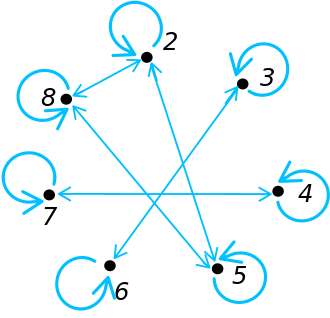
\includegraphics[scale=0.4]{../images/8.1.17.png}
\end{figure}
\end{proof}

\subsection{Exercise 18}
Let \(A = \{0, 1, 3, 4, 5, 6\}\) and define a relation $V$ on $A$ as follows: For every \(x, y \in A, x \, V \, y \iff 
5 \mid (x^2 - y^2)\).

\begin{proof}
\begin{figure}[ht!]
\centering
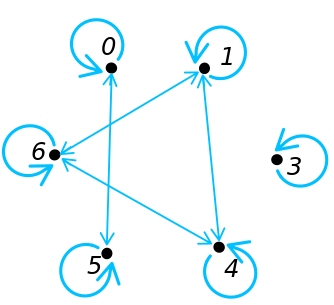
\includegraphics[scale=0.4]{../images/8.1.18.png}
\end{figure}
\end{proof}

\subsection{Exercise 19}
Let \(A = \{2, 4\}\) and \(B = \{6, 8, 10\}\) and define relations $R$ and $S$ from $A$ to $B$ as follows: For every 
\((x, y) \in A \times B, x \, R \, y \iff x \mid y\) and \( x \, S \, y \iff y - 4 = x\). State explicitly which 
ordered pairs are in \(A \times B, R, S, R \cup S\), and \(R \cap S\).

\begin{proof}
\(A \times B = \{(2, 6), (2, 8), (2, 10), (4, 6), (4, 8), (4, 10)\}\)

\(R = \{(2, 6), (2, 8), (2, 10), (4, 8)\}\), \(S = \{(2, 6), (4, 8)\}\), \(R \cup S = R, R \cap S = S\)
\end{proof}

\subsection{Exercise 20}
Let \(A = \{-1, 1, 2, 4\}\) and \(B = \{1, 2\}\) and define relations $R$ and $S$ from $A$ to $B$ as follows: For every 
\((x, y) \in A \times B, x \, R \, y \iff |x| \mid |y|\) and \(x \, S \, y \iff x - y\) is even. State explicitly 
which ordered pairs are in \(A \times B, R, S, R \cup S\), and \(R \cap S\).

\begin{proof}
\(A \times B = \{(-1, 1), (-1, 2), (1, 1), (1, 2), (2, 1), (2, 2), (4, 1), (4, 2)\}\)

\(R = \{(-1, 1), (1, 1), (2, 2)\}\), \(S = \{(-1, 1), (1, 1), (2, 2), (4, 2)\}\), \(R \cup S = S, R \cap S = R\)
\end{proof}

\subsection{Exercise 21}
Define relations $R$ and $S$ on $R$ as follows: \(R = \{(x, y) \in \R \times \R \, | \, x < y\}\) and 

\(S = \{(x, y) \in \R \times \R \, | \, x = y\}\). That is, $R$ is the “less than” relation and $S$ is the “equals” 
relation on $\R$. Graph \(R, S, R \cup S\), and \(R \cap S\) in the Cartesian plane.

\begin{proof}
The graph of the intersection of $R$ and $S$ is obtained by finding the set of all points common to both graphs. But 
there are no points for which both \(x < y\) and \(x = y\). Hence \(R \cap S = \es\) and the graph consists of no 
points at all.

\begin{figure}[ht!]
\centering
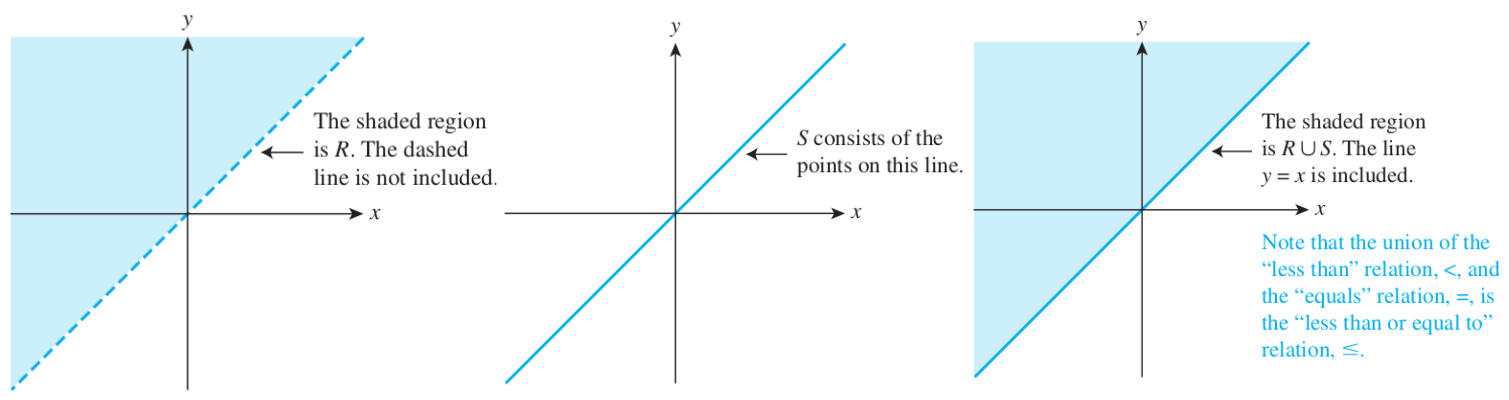
\includegraphics[scale=0.35]{../images/8.1.21.png}
\end{figure}
\end{proof}

\subsection{Exercise 22}
Define relations $R$ and $S$ on $R$ as follows: \(R = \{(x, y) \in \R \times \R \, | \, x^2 + y^2 = 4\}\) and 
\(S = \{(x, y) \in \R \times \R \, | \, x = y\}\). Graph \(R, S, R \cup S\), and \(R \cap S\) in the Cartesian plane.

\begin{proof}
\begin{figure}[ht!]
\centering
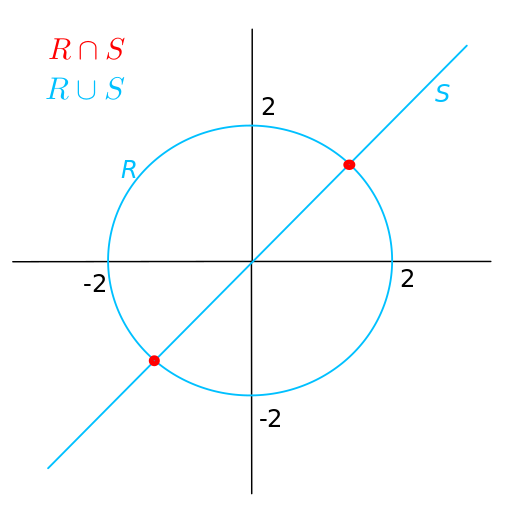
\includegraphics[scale=0.3]{../images/8.1.22.png}
\end{figure}
\end{proof}

\subsection{Exercise 23}
Define relations $R$ and $S$ on $R$ as follows: \(R = \{(x, y) \in \R \times \R \, | \, y = |x|\}\) and 
\(S = \{(x, y) \in \R \times \R \, | \, y = 1\}\). Graph \(R, S, R \cup S\), and \(R \cap S\) in the Cartesian plane.

\begin{proof}
\begin{figure}[ht!]
\centering
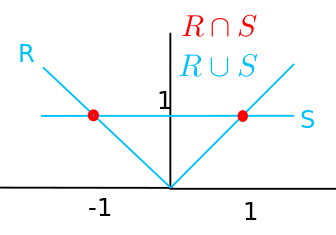
\includegraphics[scale=0.35]{../images/8.1.23.png}
\end{figure}
\end{proof}

\subsection{Exercise 24}
In Example 8.1.7 consider the query SELECT Patient\_ID\#, Name FROM S WHERE Primary\_Diagnosis = $X$. The response to 
the query is the projection onto the first two coordinates of the intersection of the database with the set 
\(A_1 \times A_2 \times A_3 \times \{X\}\).

\subsubsection{(a)}
Find the result of the query SELECT Patient\_ID\#, Name FROM S WHERE Primary\_Diagnosis = pneumonia.

\begin{proof}
574329 Tak Kurosawa, 011985 John Schmidt
\end{proof}

\subsubsection{(b)}
Find the result of the query SELECT Patient\_ID\#, Name FROM S WHERE Primary\_Diagnosis = appendicitis.

\begin{proof}
466581 Mary Lazars, 778400 Jamal Baskers
\end{proof}

\section{Exercise Set 8.2}

\subsection{Exercise 1}

\subsubsection{(a)}

\begin{proof}

\end{proof}

\subsubsection{(b)}

\begin{proof}

\end{proof}

\subsubsection{(c)}

\begin{proof}

\end{proof}

\subsubsection{(d)}

\begin{proof}

\end{proof}

\subsection{Exercise 2}

\subsubsection{(a)}

\begin{proof}

\end{proof}

\subsubsection{(b)}

\begin{proof}

\end{proof}

\subsubsection{(c)}

\begin{proof}

\end{proof}

\subsubsection{(d)}

\begin{proof}

\end{proof}

\subsection{Exercise 3}

\subsubsection{(a)}

\begin{proof}

\end{proof}

\subsubsection{(b)}

\begin{proof}

\end{proof}

\subsubsection{(c)}

\begin{proof}

\end{proof}

\subsubsection{(d)}

\begin{proof}

\end{proof}

\subsection{Exercise 4}

\subsubsection{(a)}

\begin{proof}

\end{proof}

\subsubsection{(b)}

\begin{proof}

\end{proof}

\subsubsection{(c)}

\begin{proof}

\end{proof}

\subsubsection{(d)}

\begin{proof}

\end{proof}

\subsection{Exercise 5}

\subsubsection{(a)}

\begin{proof}

\end{proof}

\subsubsection{(b)}

\begin{proof}

\end{proof}

\subsubsection{(c)}

\begin{proof}

\end{proof}

\subsubsection{(d)}

\begin{proof}

\end{proof}

\subsection{Exercise 6}

\subsubsection{(a)}

\begin{proof}

\end{proof}

\subsubsection{(b)}

\begin{proof}

\end{proof}

\subsubsection{(c)}

\begin{proof}

\end{proof}

\subsubsection{(d)}

\begin{proof}

\end{proof}

\subsection{Exercise 7}

\subsubsection{(a)}

\begin{proof}

\end{proof}

\subsubsection{(b)}

\begin{proof}

\end{proof}

\subsubsection{(c)}

\begin{proof}

\end{proof}

\subsubsection{(d)}

\begin{proof}

\end{proof}

\subsection{Exercise 8}

\subsubsection{(a)}

\begin{proof}

\end{proof}

\subsubsection{(b)}

\begin{proof}

\end{proof}

\subsubsection{(c)}

\begin{proof}

\end{proof}

\subsubsection{(d)}

\begin{proof}

\end{proof}

\subsection{Exercise 9}

\begin{proof}

\end{proof}

\subsection{Exercise 10}

\begin{proof}

\end{proof}

\subsection{Exercise 11}

\begin{proof}

\end{proof}

\subsection{Exercise 12}

\begin{proof}

\end{proof}

\subsection{Exercise 13}

\begin{proof}

\end{proof}

\subsection{Exercise 14}

\begin{proof}

\end{proof}

\subsection{Exercise 15}

\begin{proof}

\end{proof}

\subsection{Exercise 16}

\begin{proof}

\end{proof}

\subsection{Exercise 17}

\begin{proof}

\end{proof}

\subsection{Exercise 18}

\begin{proof}

\end{proof}

\subsection{Exercise 19}

\begin{proof}

\end{proof}

\subsection{Exercise 20}

\begin{proof}

\end{proof}

\subsection{Exercise 21}

\begin{proof}

\end{proof}

\subsection{Exercise 22}

\begin{proof}

\end{proof}

\subsection{Exercise 23}

\begin{proof}

\end{proof}

\subsection{Exercise 24}

\begin{proof}

\end{proof}

\subsection{Exercise 25}

\begin{proof}

\end{proof}

\subsection{Exercise 26}

\begin{proof}

\end{proof}

\subsection{Exercise 27}

\begin{proof}

\end{proof}

\subsection{Exercise 28}

\begin{proof}

\end{proof}

\subsection{Exercise 29}

\begin{proof}

\end{proof}

\subsection{Exercise 30}

\begin{proof}

\end{proof}

\subsection{Exercise 31}

\begin{proof}

\end{proof}

\subsection{Exercise 32}

\begin{proof}

\end{proof}

\subsection{Exercise 33}

\begin{proof}

\end{proof}

\subsection{Exercise 34}

\begin{proof}

\end{proof}

\subsection{Exercise 35}

\begin{proof}

\end{proof}

\subsection{Exercise 36}

\begin{proof}

\end{proof}

\subsection{Exercise 37}

\begin{proof}

\end{proof}

\subsection{Exercise 38}

\begin{proof}

\end{proof}

\subsection{Exercise 39}

\begin{proof}

\end{proof}

\subsection{Exercise 40}

\begin{proof}

\end{proof}

\subsection{Exercise 41}

\begin{proof}

\end{proof}

\subsection{Exercise 42}

\begin{proof}

\end{proof}

\subsection{Exercise 43}

\begin{proof}

\end{proof}

\subsection{Exercise 44}

\begin{proof}

\end{proof}

\subsection{Exercise 45}

\begin{proof}

\end{proof}

\subsection{Exercise 46}

\begin{proof}

\end{proof}

\subsection{Exercise 47}

\begin{proof}

\end{proof}

\subsection{Exercise 48}

\begin{proof}

\end{proof}

\subsection{Exercise 49}

\begin{proof}

\end{proof}

\subsection{Exercise 50}

\begin{proof}

\end{proof}

\subsection{Exercise 51}

\begin{proof}

\end{proof}

\subsection{Exercise 52}

\begin{proof}

\end{proof}

\subsection{Exercise 53}

\begin{proof}

\end{proof}

\subsection{Exercise 54}

\begin{proof}

\end{proof}

\subsection{Exercise 55}

\begin{proof}

\end{proof}

\subsection{Exercise 56}

\begin{proof}

\end{proof}

\section{Exercise Set 8.3}

\subsection{Exercise 1}

\subsubsection{(a)}

\begin{proof}

\end{proof}

\subsubsection{(b)}

\begin{proof}

\end{proof}

\subsubsection{(c)}

\begin{proof}

\end{proof}

\subsubsection{(d)}

\begin{proof}

\end{proof}

\subsection{Exercise 2}

\subsubsection{(a)}

\begin{proof}

\end{proof}

\subsubsection{(b)}

\begin{proof}

\end{proof}

\subsubsection{(c)}

\begin{proof}

\end{proof}

\subsection{Exercise 3}

\begin{proof}

\end{proof}

\subsection{Exercise 4}

\begin{proof}

\end{proof}

\subsection{Exercise 5}

\begin{proof}

\end{proof}

\subsection{Exercise 6}

\begin{proof}

\end{proof}

\subsection{Exercise 7}

\begin{proof}

\end{proof}

\subsection{Exercise 8}

\begin{proof}

\end{proof}

\subsection{Exercise 9}

\begin{proof}

\end{proof}

\subsection{Exercise 10}

\begin{proof}

\end{proof}

\subsection{Exercise 11}

\begin{proof}

\end{proof}

\subsection{Exercise 12}

\begin{proof}

\end{proof}

\subsection{Exercise 13}

\begin{proof}

\end{proof}

\subsection{Exercise 14}

\begin{proof}

\end{proof}

\subsection{Exercise 15}

\subsubsection{(a)}

\begin{proof}

\end{proof}

\subsubsection{(b)}

\begin{proof}

\end{proof}

\subsubsection{(c)}

\begin{proof}

\end{proof}

\subsubsection{(d)}

\begin{proof}

\end{proof}

\subsection{Exercise 16}

\subsubsection{(a)}

\begin{proof}

\end{proof}

\subsubsection{(b)}

\begin{proof}

\end{proof}

\subsection{Exercise 17}

\subsubsection{(a)}

\begin{proof}

\end{proof}

\subsubsection{(b)}

\begin{proof}

\end{proof}

\subsection{Exercise 18}

\subsubsection{(a)}

\begin{proof}

\end{proof}

\subsubsection{(b)}

\begin{proof}

\end{proof}

\subsection{Exercise 19}

\subsubsection{(a)}

\begin{proof}

\end{proof}

\subsubsection{(b)}

\begin{proof}

\end{proof}

\subsection{Exercise 20}

\begin{proof}

\end{proof}

\subsection{Exercise 21}

\begin{proof}

\end{proof}

\subsection{Exercise 22}

\begin{proof}

\end{proof}

\subsection{Exercise 23}

\begin{proof}

\end{proof}

\subsection{Exercise 24}

\begin{proof}

\end{proof}

\subsection{Exercise 25}

\begin{proof}

\end{proof}

\subsection{Exercise 26}

\begin{proof}

\end{proof}

\subsection{Exercise 27}

\begin{proof}

\end{proof}

\subsection{Exercise 28}

\begin{proof}

\end{proof}

\subsection{Exercise 29}

\begin{proof}

\end{proof}

\subsection{Exercise 30}

\begin{proof}

\end{proof}

\subsection{Exercise 31}

\begin{proof}

\end{proof}

\subsection{Exercise 32}

\begin{proof}

\end{proof}

\subsection{Exercise 33}

\begin{proof}

\end{proof}

\subsection{Exercise 34}

\begin{proof}

\end{proof}

\subsection{Exercise 35}

\begin{proof}

\end{proof}

\subsection{Exercise 36}

\begin{proof}

\end{proof}

\subsection{Exercise 37}

\begin{proof}

\end{proof}

\subsection{Exercise 38}

\begin{proof}

\end{proof}

\subsection{Exercise 39}

\begin{proof}

\end{proof}

\subsection{Exercise 40}

\begin{proof}

\end{proof}

\subsection{Exercise 41}

\begin{proof}

\end{proof}

\subsection{Exercise 42}

\subsubsection{(a)}

\begin{proof}

\end{proof}

\subsubsection{(b)}

\begin{proof}

\end{proof}

\subsubsection{(c)}

\begin{proof}

\end{proof}

\subsubsection{(d)}

\begin{proof}

\end{proof}

\subsection{Exercise 43}

\subsubsection{(a)}

\begin{proof}

\end{proof}

\subsubsection{(b)}

\begin{proof}

\end{proof}

\subsubsection{(c)}

\begin{proof}

\end{proof}

\subsubsection{(d)}

\begin{proof}

\end{proof}

\subsubsection{(e)}

\begin{proof}

\end{proof}

\subsubsection{(f)}

\begin{proof}

\end{proof}

\subsection{Exercise 44}

\subsubsection{(a)}

\begin{proof}

\end{proof}

\subsubsection{(b)}

\begin{proof}

\end{proof}

\subsubsection{(c)}

\begin{proof}

\end{proof}

\subsubsection{(d)}

\begin{proof}

\end{proof}

\subsubsection{(e)}

\begin{proof}

\end{proof}

\subsubsection{(f)}

\begin{proof}

\end{proof}

\subsubsection{(g)}

\begin{proof}

\end{proof}

\subsection{Exercise 45}

\begin{proof}

\end{proof}

\subsection{Exercise 46}

\begin{proof}

\end{proof}

\subsection{Exercise 47}

\subsubsection{(a)}

\begin{proof}

\end{proof}

\subsubsection{(b)}

\begin{proof}

\end{proof}

\subsubsection{(c)}

\begin{proof}

\end{proof}

\subsubsection{(d)}

\begin{proof}

\end{proof}

\subsubsection{(e)}

\begin{proof}

\end{proof}

\subsubsection{(f)}

\begin{proof}

\end{proof}

\subsubsection{(g)}

\begin{proof}

\end{proof}

\section{Exercise Set 8.4}

\subsection{Exercise 1}

\subsubsection{(a)}

\begin{proof}

\end{proof}

\subsubsection{(b)}

\begin{proof}

\end{proof}

\subsection{Exercise 2}

\subsubsection{(a)}

\begin{proof}

\end{proof}

\subsubsection{(b)}

\begin{proof}

\end{proof}

\subsection{Exercise 3}

\subsubsection{(a)}

\begin{proof}

\end{proof}

\subsubsection{(b)}

\begin{proof}

\end{proof}

\subsubsection{(c)}

\begin{proof}

\end{proof}

\subsubsection{(d)}

\begin{proof}

\end{proof}

\subsubsection{(e)}

\begin{proof}

\end{proof}

\subsection{Exercise 4}

\subsubsection{(a)}

\begin{proof}

\end{proof}

\subsubsection{(b)}

\begin{proof}

\end{proof}

\subsubsection{(c)}

\begin{proof}

\end{proof}

\subsubsection{(d)}

\begin{proof}

\end{proof}

\subsubsection{(e)}

\begin{proof}

\end{proof}

\subsection{Exercise 5}

\begin{proof}

\end{proof}

\subsection{Exercise 6}

\begin{proof}

\end{proof}

\subsection{Exercise 7}

\subsubsection{(a)}

\begin{proof}

\end{proof}

\subsubsection{(b)}

\begin{proof}

\end{proof}

\subsubsection{(c)}

\begin{proof}

\end{proof}

\subsubsection{(d)}

\begin{proof}

\end{proof}

\subsubsection{(e)}

\begin{proof}

\end{proof}

\subsection{Exercise 8}

\subsubsection{(a)}

\begin{proof}

\end{proof}

\subsubsection{(b)}

\begin{proof}

\end{proof}

\subsubsection{(c)}

\begin{proof}

\end{proof}

\subsubsection{(d)}

\begin{proof}

\end{proof}

\subsubsection{(e)}

\begin{proof}

\end{proof}

\subsection{Exercise 9}

\subsubsection{(a)}

\begin{proof}

\end{proof}

\subsubsection{(b)}

\begin{proof}

\end{proof}

\subsection{Exercise 10}

\begin{proof}

\end{proof}

\subsection{Exercise 11}

\begin{proof}

\end{proof}

\subsection{Exercise 12}

\subsubsection{(a)}

\begin{proof}

\end{proof}

\subsubsection{(b)}

\begin{proof}

\end{proof}

\subsection{Exercise 13}

\subsubsection{(a)}

\begin{proof}

\end{proof}

\subsubsection{(b)}

\begin{proof}

\end{proof}

\subsection{Exercise 14}

\begin{proof}

\end{proof}

\subsection{Exercise 15}

\begin{proof}

\end{proof}

\subsection{Exercise 16}

\begin{proof}

\end{proof}

\subsection{Exercise 17}

\begin{proof}

\end{proof}

\subsection{Exercise 18}

\begin{proof}

\end{proof}

\subsection{Exercise 19}

\begin{proof}

\end{proof}

\subsection{Exercise 20}

\begin{proof}

\end{proof}

\subsection{Exercise 21}

\begin{proof}

\end{proof}

\subsection{Exercise 22}

\begin{proof}

\end{proof}

\subsection{Exercise 23}

\begin{proof}

\end{proof}

\subsection{Exercise 24}

\begin{proof}

\end{proof}

\subsection{Exercise 25}

\begin{proof}

\end{proof}

\subsection{Exercise 26}

\begin{proof}

\end{proof}

\subsection{Exercise 27}

\begin{proof}

\end{proof}

\subsection{Exercise 28}

\begin{proof}

\end{proof}

\subsection{Exercise 29}

\begin{proof}

\end{proof}

\subsection{Exercise 30}

\begin{proof}

\end{proof}

\subsection{Exercise 31}

\subsubsection{(a)}

\begin{proof}

\end{proof}

\subsubsection{(b)}

\begin{proof}

\end{proof}

\subsubsection{(c)}

\begin{proof}

\end{proof}

\subsection{Exercise 32}

\subsubsection{(a)}

\begin{proof}

\end{proof}

\subsubsection{(b)}

\begin{proof}

\end{proof}

\subsection{Exercise 33}

\begin{proof}

\end{proof}

\subsection{Exercise 34}

\begin{proof}

\end{proof}

\subsection{Exercise 35}

\begin{proof}

\end{proof}

\subsection{Exercise 36}

\begin{proof}

\end{proof}

\subsection{Exercise 37}

\begin{proof}

\end{proof}

\subsection{Exercise 38}

\begin{proof}

\end{proof}

\subsection{Exercise 39}

\begin{proof}

\end{proof}

\subsection{Exercise 40}

\begin{proof}

\end{proof}

\subsection{Exercise 41}

\subsubsection{(a)}

\begin{proof}

\end{proof}

\subsubsection{(b)}

\begin{proof}

\end{proof}

\subsection{Exercise 42}

\begin{proof}

\end{proof}

\subsection{Exercise 43}

\begin{proof}

\end{proof}

\section{Exercise Set 8.5}

\subsection{Exercise 1}

\subsubsection{(a)}

\begin{proof}

\end{proof}

\subsubsection{(b)}

\begin{proof}

\end{proof}

\subsubsection{(c)}

\begin{proof}

\end{proof}

\subsubsection{(d)}

\begin{proof}

\end{proof}

\subsection{Exercise 2}

\begin{proof}

\end{proof}

\subsection{Exercise 3}

\begin{proof}

\end{proof}

\subsection{Exercise 4}

\begin{proof}

\end{proof}

\subsection{Exercise 5}

\begin{proof}

\end{proof}

\subsection{Exercise 6}

\begin{proof}

\end{proof}

\subsection{Exercise 7}

\begin{proof}

\end{proof}

\subsection{Exercise 8}

\begin{proof}

\end{proof}

\subsection{Exercise 9}

\begin{proof}

\end{proof}

\subsection{Exercise 10}

\begin{proof}

\end{proof}

\subsection{Exercise 11}

\subsubsection{(a)}

\begin{proof}

\end{proof}

\subsubsection{(b)}

\begin{proof}

\end{proof}

\subsubsection{(c)}

\begin{proof}

\end{proof}

\subsubsection{(d)}

\begin{proof}

\end{proof}

\subsubsection{(e)}

\begin{proof}

\end{proof}

\subsubsection{(f)}

\begin{proof}

\end{proof}

\subsubsection{(g)}

\begin{proof}

\end{proof}

\subsection{Exercise 12}

\begin{proof}

\end{proof}

\subsection{Exercise 13}

\begin{proof}

\end{proof}

\subsection{Exercise 14}

\subsubsection{(a)}

\begin{proof}

\end{proof}

\subsubsection{(b)}

\begin{proof}

\end{proof}

\subsection{Exercise 15}

\begin{proof}

\end{proof}

\subsection{Exercise 16}

\subsubsection{(a)}

\begin{proof}

\end{proof}

\subsubsection{(b)}

\begin{proof}

\end{proof}

\subsection{Exercise 17}

\begin{proof}

\end{proof}

\subsection{Exercise 18}

\begin{proof}

\end{proof}

\subsection{Exercise 19}

\begin{proof}

\end{proof}

\subsection{Exercise 20}

\begin{proof}

\end{proof}

\subsection{Exercise 21}

\subsubsection{(a)}

\begin{proof}

\end{proof}

\subsubsection{(b)}

\begin{proof}

\end{proof}

\subsection{Exercise 22}

\begin{proof}

\end{proof}

\subsection{Exercise 23}

\begin{proof}

\end{proof}

\subsection{Exercise 24}

\begin{proof}

\end{proof}

\subsection{Exercise 25}

\begin{proof}

\end{proof}

\subsection{Exercise 26}

\begin{proof}

\end{proof}

\subsection{Exercise 27}

\begin{proof}

\end{proof}

\subsection{Exercise 28}

\begin{proof}

\end{proof}

\subsection{Exercise 29}

\begin{proof}

\end{proof}

\subsection{Exercise 30}

\subsubsection{(a)}

\begin{proof}

\end{proof}

\subsubsection{(b)}

\begin{proof}

\end{proof}

\subsubsection{(c)}

\begin{proof}

\end{proof}

\subsubsection{(d)}

\begin{proof}

\end{proof}

\subsection{Exercise 31}

\begin{proof}

\end{proof}

\subsection{Exercise 32}

\begin{proof}

\end{proof}

\subsection{Exercise 33}

\begin{proof}

\end{proof}

\subsection{Exercise 34}

\begin{proof}

\end{proof}

\subsection{Exercise 35}

\begin{proof}

\end{proof}

\subsection{Exercise 36}

\begin{proof}

\end{proof}

\subsection{Exercise 37}

\begin{proof}

\end{proof}

\subsection{Exercise 38}

\begin{proof}

\end{proof}

\subsection{Exercise 39}

\begin{proof}

\end{proof}

\subsection{Exercise 40}

\subsubsection{(a)}

\begin{proof}

\end{proof}

\subsubsection{(b)}

\begin{proof}

\end{proof}

\subsection{Exercise 41}

\subsubsection{(a)}

\begin{proof}

\end{proof}

\subsubsection{(b)}

\begin{proof}

\end{proof}

\subsection{Exercise 42}

\begin{proof}

\end{proof}

\subsection{Exercise 43}

\begin{proof}

\end{proof}

\subsection{Exercise 44}

\begin{proof}

\end{proof}

\subsection{Exercise 45}

\begin{proof}

\end{proof}

\subsection{Exercise 46}

\begin{proof}

\end{proof}

\subsection{Exercise 47}

\begin{proof}

\end{proof}

\subsection{Exercise 48}

\begin{proof}

\end{proof}

\subsection{Exercise 49}

\subsubsection{(a)}

\begin{proof}

\end{proof}

\subsubsection{(b)}

\begin{proof}

\end{proof}

\subsection{Exercise 50}

\subsubsection{(a)}

\begin{proof}

\end{proof}

\subsubsection{(b)}

\begin{proof}

\end{proof}

\subsection{Exercise 51}

\subsubsection{(a)}

\begin{proof}

\end{proof}

\subsubsection{(b)}

\begin{proof}

\end{proof}

\end{document}
